%
% Requerimientos de tokens, análisis y diseño de generación de tokens.
% Proyecto Lovelace.
%

\subsection{Requerimientos}

En \cite{pci_tokens}, el \gls{gl:pci} \gls{gl:ssc} divide a los
\glspl{gl:token} en reversibles e irreversibles. A su vez, los reversibles se
dividen en criptográficos y en no criptográficos; mientras que los
irreversibles se dividen en autenticables y no autenticables (figura
\ref{fig:division_tokens}).

\begin{figure}[H]
  \begin{center}
    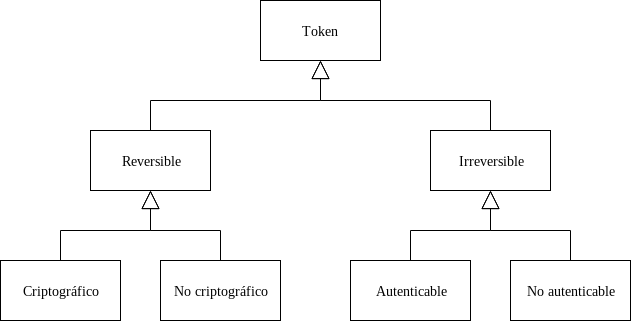
\includegraphics[width=0.75\linewidth]
      {contenidos/analisis_y_disenio/tokens/requerimientos/diagramas/clasificacion.png}
    \caption{Clasificación de los \glspl{gl:token}.}
    \label{fig:division_tokens}
  \end{center}
\end{figure}

En esta sección se explica cada una de las categorías y se analizan los
requerimientos que deben tener. Para comenzar, se enlistan los requerimientos
aplicables a todos los \glspl{gl:token}, sin importar en qué categoría estén:

%\requerimiento{tokens}{seguridad}{
%  Un adversario con acceso a los \glspl{gl:token} no debe de ser capaz de
%  obtener los \gls{gl:pan} asociados.
%}

\begin{itemize}
  % GT1 Es específico a productos de hardware.
  % GT2 se lo chutaron.
  % GT3 Validación FIPS que debe cumplir el software; fuera de alcance.

  % GT4 - Resistensia a texto claro conocido.
  \item Un atacante con acceso a múltiples pares de \glspl{gl:token} y
    \gls{gl:pan} no debe de ser capaz de determinar otros \gls{gl:pan} a partir
    de solamente \glspl{gl:token}. En otras palabras, los \glspl{gl:token}
    deben ser resistentes a ataques con texto en claro conocido (sección
    \ref{sec:criptoanalisis}).

  % GT5 - Resistencia a sólo texto cifrado.
  % Me parece que esto es reduntante: si GT4 ya estableció la necesidad de
  % resistencia a texto claro conocido, la resistencia a sólo texto cifrado
  % ya va incluida. De hecho, en la misma redacción de GT5 incluyen claramente
  % a GT4 con una disyunción.
  % Creo que ya había leído esto mismo en alguno de los artículos que nos pasó
  % Sandra.
  \item Recuperar un \gls{gl:pan} a partir de un \gls{gl:token} debe de ser
    \gls{gl:computacionalmente_no_factible} (resistencia a ataques con sólo
    texto cifrado, sección \ref{sec:criptoanalisis}).

  % GT6 Detección de anomalías.
  % ¿Requerimiento de API web?
  \item Se deben de implementar monitoreos que permitan detectar
     irregularidades en el sistema (anomalías, funcionamientos erróneos,
     comportamientos sospechosos). El producto debe registrar dichos eventos y
     avisar al personal correspondiente.

  % GT7 Distinción entre tokens y PAN.
  \item Se debe contar con un mecanismo para distinguir entre \glspl{gl:token}
    y \gls{gl:pan}. Los proveedores del servicio de tokenización deben
    compartir este mecanismo con la entidad (o entidades) que usa los
    \glspl{gl:token}.

  % GT8 Guía de instalación; fuera de alcance. ¿Documentación de API web?
  % de cualquier forma, es requerimiento de api web.
  % GT9 Integridad de ejecutables; fuera de alcance.
  % GT10 Autenticación de usuarios; requerimiento de api web.

  % GT11 Mapeos de token a token prohibidos.
  \item No se debe poder pasar de un primer \gls{gl:token} válido a un segundo,
    también válido; forzosamente debe existir un estado intermedio: del primer
    \gls{gl:token} se pasa al \gls{gl:pan} correspondiente (operación de
    detokenización) y de este se pasa al segundo \gls{gl:token}.

  % GT12 Protección contra vulnerabilidades comunes.
  \item Se deben implementar medidas en contra de las vulnerabilidades de
    seguridad más comunes (\cite{dss_pa}, requerimiento 5.2). Algunas de estas
    medidas pueden ser el uso de herramientas de análisis de código estático,
    o el uso de lenguajes de programación especializados.

  % GT13 Primitivas criptográficas usadas
  % También se habla sobre un documento de validación estadísitca, fuera de
  % alcance.
  \item Las primitivas criptográficas que se usen deben estar basadas en
    estándares nacionales (Estados Unidos) o internacionales (e. g.
    \gls{gl:aes}).
\end{itemize}

Los \glspl{gl:token} irreversibles no pueden, bajo ninguna circunstancia, ser
reconvertidos al \gls{gl:pan} original. Esta restricción aplica tanto para
cualquier entidad en el entorno del negocio (comerciante, proveedor de
\glspl{gl:token}, banco) como para cualquier posible atacante. Dados un
\gls{gl:pan} y un \gls{gl:token}, los identificables permiten validar cuando el
primero fue utilizado para la creación del segundo, mientras que los no
identificables, no.

% TODO: ¿Para qué demonios sirven los no identificables?

% TODO: este párrafo me está dando problemas. No quiero copiar tal cuál la
% clasificación del PCI sin manifestar disconformidad, pero tampoco quiero
% entrar en demasiados detalles aún sobre las propias implementaciones
% (las cuales, evidentemente, sí son criptográficas).

La clasificación del \gls{gl:pci} \gls{gl:ssc} con respecto a los reversibles
resulta un poco confusa (esto ya ha sido señalado antes, \cite{doc_sandra}).
Establece que los criptográficos son generados utilizando
\gls{gl:criptografia_fuerte}, el \gls{gl:pan} nunca se almacena, solamente se
guarda una llave; los no criptográficos guardan la relación entre
\glspl{gl:token} y \gls{gl:pan} en una base de datos. El problema está en que
no se menciona \textit{cómo} generar los no criptográficos. A pesar del nombre,
los métodos más comunes para esta categoría ocupan primitivas criptográficas
(e. g. generadores pseudoaleatorios); además de que, en una implementación
real, para poder cumplir con el \gls{gl:pci} \gls{gl:dss}, la propia base de
datos debe de estar cifrada \cite{pci_dss}.

%
% Requerimientos para tokens irreversibles,
% análisis y diseño de generación de tokens.
% Proyecto Lovelace.
%

\subsection{Irreversibles}

% IT1A
\requerimientoConClasificacion
{Sobre la generación de 
  \texorpdfstring{\glspl{gl:token}}{tokens} (irreversibles)}
{clasificacion:algoritmos}
{
  El mecanismo utilizado para la generación de los \glspl{gl:token}
  no es reversible (o improbable).
}

% IT1A-1
\subrequerimiento[rq_pci:ir_mecanismo_generador]
{Sobre el mecanismo generador (irreversibles)}
{
  El proceso para crear \glspl{gl:token} clasificado como irreversible
  debe asegurar que el mecanismo, proceso o algoritmo utilizado para
  crear el \gls{gl:token} no sea reversible. Si una función hash (véase
  sección~\ref{sec:hash}) es utilizada, esta debe ser una
  \gls{gl:primitiva_criptografica} y utilizar una llave secreta $k$ tal que
  el mero conocimiento de la función hash no permita la creación de un
  \gls{gl:oraculo}.
}

% IT1A-2
\subrequerimiento[rq_pci:ir_contenido_en_claro]
{Contenido en claro (irreversibles)}
{
  Los \glspl{gl:token} irreversibles no deben contener dígitos en claro del
  \gls{gl:pan} original, excepto que estos dígitos sean una coincidencia.
}

% IT1A-3
\subrequerimiento[rq_pci:ir_diccionario_imposible]
{Creación de un diccionario (irreversibles)}
{
  La creación de una tabla o \textit{diccionario} de \glspl{gl:token}
  estáticos debería ser imposible, o, al menos, al punto de satisfacer que
  la probabilidad de predecir correctamente el \gls{gl:pan} sea menor que
  $\frac{1}{10^6}$.
}

% IT1A-4
\subrequerimiento[rq_pci:ir_busqueda_exhaustiva]
{Sobre el proceso de autenticación (irreversibles)}
{
  En el caso de los \glspl{gl:token} autenticables, el proceso de
  autenticación no debe revelar información suficiente para realizar
  búsquedas, excepto una exhaustiva (\gls{gl:pan} por \gls{gl:pan}) y se
  deben implementar controles para detectar estas últimas.
}

%En la tabla~\ref{resumen_irreversibles} se clasifican los requerimientos
%que en el documento del \gls{gl:pci} \gls{gl:ssc}~\cite{pci_tokens} están
%catalogados como irreversibles. En la lista de este documento se procura no
%hacer tal división, para evitar las repeticiones en exceso que~\cite{pci_tokens}
%manifiesta en algunas ocasiones. Por ejemplo, el requerimiento
%\cite{rq_pci:manejo_de_llaves} es aplicable tanto a los irreversibles como a
%los reversibles criptográficos (y de hecho también a los no criptográficos, dado
%que ahí también se ocupan llaves en la mayoría de los casos), sin embargo,
%en las recomendaciones de \gls{gl:pci} \gls{gl:ssc} se manejan dos versiones
%de lo mismo.

%
% Requerimientos para tokens criptográficos reversibles,
% análisis y diseño de generación de tokens.
% Proyecto Lovelace.
%

\subsection{Criptográficos reversibles}

% RC1B
% TODO: el documento explica por qué esta cantidad; aún no lo entiendo.
\requerimiento{Probabilidad de adivinar relaciones (criptográficos)}
{
  La probabilidad de adivinar la relación entre un \gls{gl:token} y un
  \gls{gl:pan} debe de ser menor que $ 1 $ en $ 10^6 $.
}

% RC1B-1
\subrequerimiento[rq_pci:cr_distribucion_uniforme]
{Distribución uniforme (criptográficos)}
{
  Para un \gls{gl:pan} dado, todos los \glspl{gl:token} deben ser
  equiprobables; esto es, el mecanismo tokenizador no debe exhibir
  tendencias probabilísticas que lo expongan a ataques estadísticos.
}

% RC1B-2 permutación aleatoria
% TODO: ¿Cuál es la diferencia entre una «permutación aleatoria» y una
% «permutación aleatoria fuerte»?
% Si el mapeo es entre dos espacios distintos... ya no se llama
% permutación, ¿o sí?
\subrequerimiento[rq_pci:cr_permutacion_aleatoria]
{Permutación aleatoria (criptográficos)}
{
  El método de tokenización debe actuar como una familia de
  \glspl{gl:permutacion} aleatoria desde el espacio de \gls{gl:pan} al
  espacio de \glspl{gl:token}.
}

% RC1B-3
\subrequerimiento[rq_pci:cr_cambio_de_llave]
{Cambio de llave (criptográficos)}
{
  Un cambio en la llave se debe ver reflejado en un cambio en el
  \gls{gl:token} resultado.
}

% RC1B-4
\subrequerimiento[rq_pci:cr_cambio_de_pan]
{Cambio de \gls{gl:pan} (criptográficos)}
{
  Un cambio en el \gls{gl:pan} se debe ver reflejado en un cambio en el
  \gls{gl:token} resultado.
}

% RC1B-5
\subrequerimiento[rq_pci:cr_aleatoriedad_digitos]
{Verificación de la aleatoriedad (criptográficos)}
{
  Se debe tener un medio para verificar de forma práctica la aleatorización
  de dígitos, de acuerdo a lo establecido en \gls{gl:nist} 800-90A
 ~\cite{nist_aleatorios}.
}

% RC1C almacenamiento duplicado
% Este no lo entiendo: primero, ¿qué no se suponía que en los criptográficos
% nunca se almacenaba el token?; segundo, aún suponiendo que este
% requerimiento fuera en realidad para los no criptográficos, ¿Cuál es la
% diferencia entre guardar el PAN completo y guardar el PAN truncado?
\requerimiento[rq_pci:cr_almacenamiento_tokens]
{Almacenamiento de tokens (criptográficos)}
{
  Los \glspl{gl:token} generados no se deben almacenar en ningún punto del
  sistema.
}

El requerimiento anterior (\hipervinculo{rq_pci:cr_almacenamiento_tokens},
RC1C en~\cite{pci_tokens}) es un tanto difícil de interpretar; la versión
original establece: \textit{los \glspl{gl:token} basados en el \gls{gl:pan}
completo no se deben almacenar si el producto tokenizador también almacena
su \gls{gl:pan} truncado correspondiente}. Es un requerimiento de los
criptográficos reversibles, por lo que el \gls{gl:token} no se debería
almacenar bajo ninguna circunstancia (según la propia clasificación del
\gls{gl:pci} \gls{gl:ssc}); la redacción del requerimiento se cambió para
reflejar este hecho.

% RC4A
\requerimiento[rq_pci:cr_administracion_llaves]
{Seguridad de la administración de llaves (criptográficos)}
{
  Todas la operaciones sobre la administración de las llaves criptográficas
  deben realizarse en un dispositivo criptográfico seguro y aprobado: el
  \gls{gl:pci} \gls{gl:ssc} se encarga de hacer validaciones; también puede ser
  cualquier dispositivo validado por \gls{gl:fips} 140-2 nivel 3 o superior
 ~\cite{nist_modulos_criptograficos} o por la \gls{gl:iso} 13491-1.
}

% RC4C-1 y 2
\requerimiento[rq_pci:cr_longitud_llaves]
{Sobre la longitud de las llaves (criptográficos)}
{
  Las llaves para \textit{tokenizar} deben tener una
  \gls{gl:fuerza_efectiva} de, al menos, 128 bits. Cualquier llave utilizada
  para proteger o para derivar la llave del \gls{gl:token} debe de ser de igual
  o mayor \gls{gl:fuerza_efectiva}.
}

% RC4D
\requerimiento[rq_pci:cr_independencia_estadistica]
{Independencia estadística (criptográficos)}
{
  Si el espacio de llaves es usado para producir \glspl{gl:token} es dos
  contextos distintos (p. ej. para distintos comerciantes), estas deben ser
  \glspl{gl:estidisticamente_independiente}.
}

%
% Requerimientos para tokens no criptográficos reversibles,
% análisis y diseño de generación de tokens.
% Proyecto Lovelace.
%

\subsubsection{No criptográficos reversibles}

